%\documentclass[aps,prd,nofootinbib]{revtex4-1}
\documentclass[preprint,notitlepage,nofootinbib]{revtex4-1}
\usepackage{amsmath}
\usepackage{graphicx}
\usepackage{subfig}
\usepackage{epsfig}
\usepackage{listings}
\usepackage[hidelinks,hyperfootnotes=false,bookmarks=false]{hyperref}
\begin{document}
\title{Problem Set 1 - G6080}
\author{Victor Genty}
%\affiliation{Department of Physics, Duke University, Durham, NC 27707, USA}
\date{\today}
%\begin{abstract}
%\end{abstract}
\maketitle
\section{Problem 1}
%\label{sec1}
The cosine recursion formula  was implemented in C++ double precision and plotted for various values of $N$ at constant $x$. The error function for an accuracy of $\epsilon_c = 10^{-15}$ in the initial guess is plotted as well as the ratio of cosine to the error function. We find that as N is increased from $N=10^{2}$ to $N=10^8$ the relative error in cosine from recursion follows the expected pattern and the {\it ratio} of the recursion cosine to the error function reveals an increasing value of $\epsilon_c$ with $N$.
\begin{figure}[h]
  \centering
\subfloat[][]{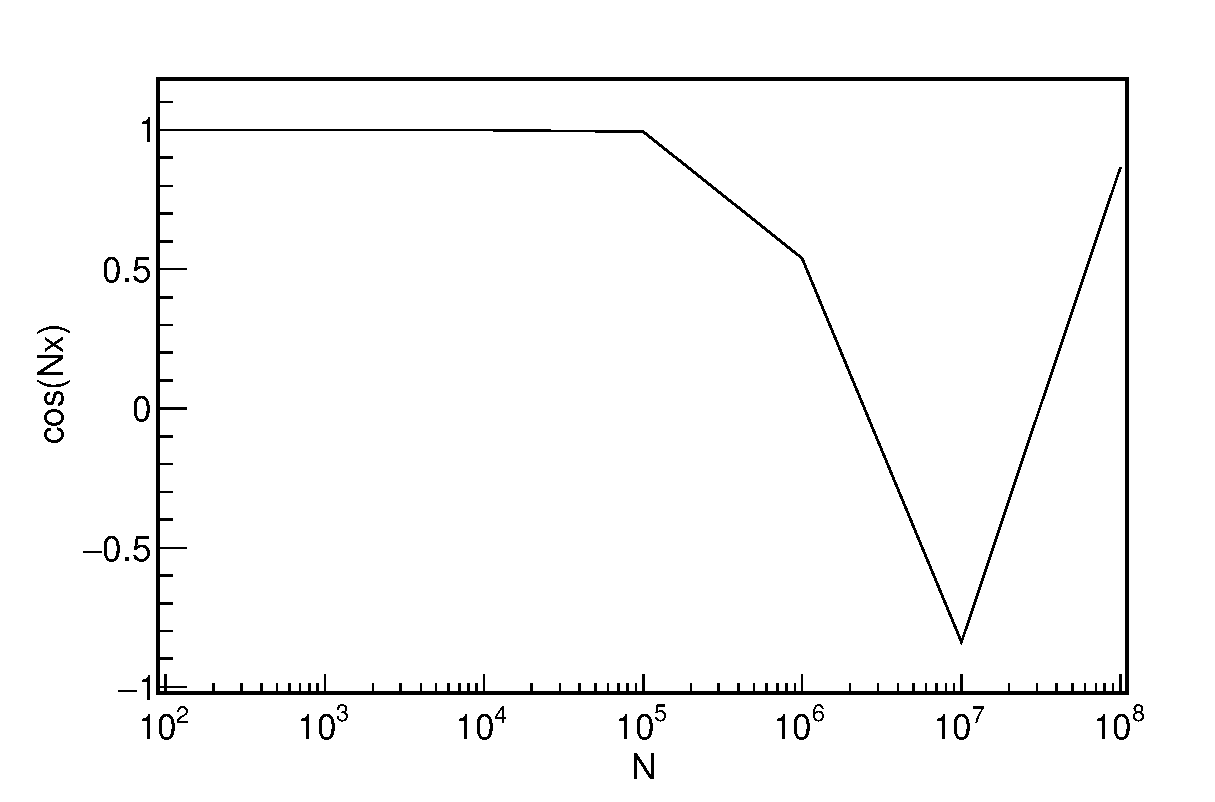
\includegraphics[width=0.5\textwidth]{figures/1a_cos.eps}}
\subfloat[][]{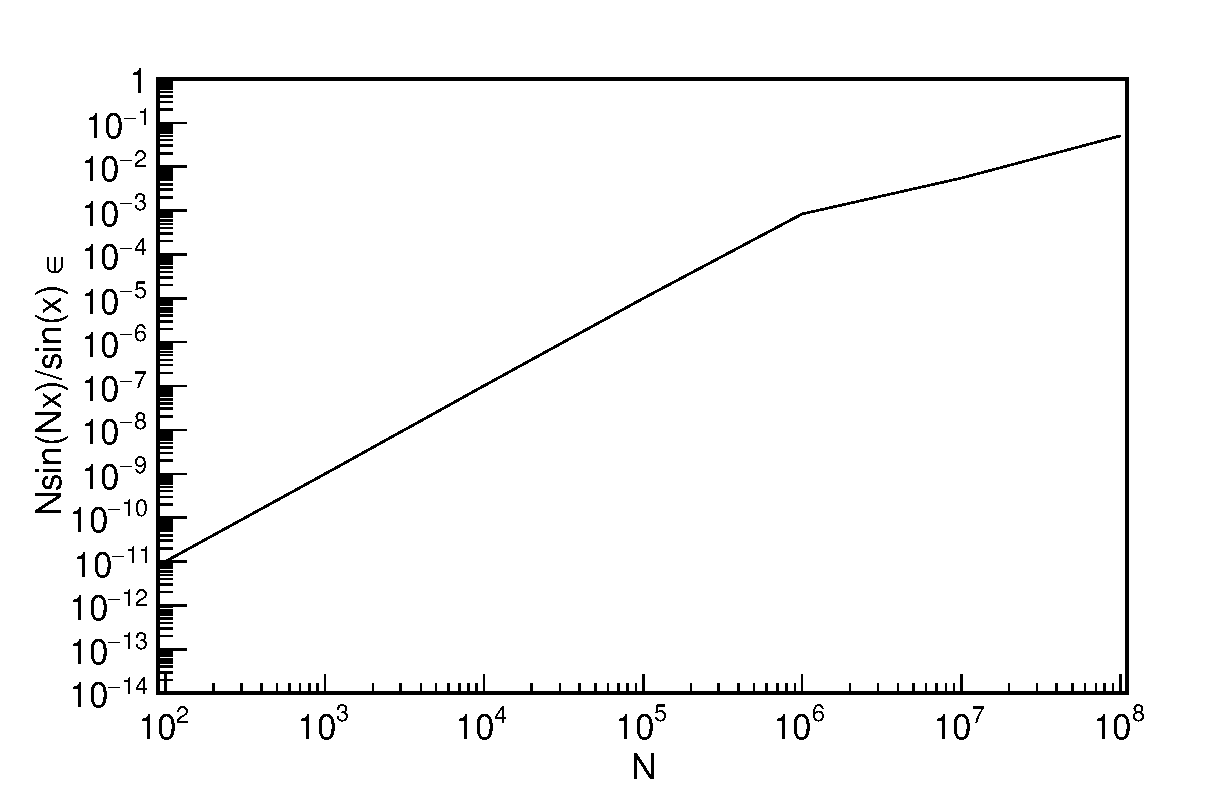
\includegraphics[width=0.5\textwidth]{figures/1a_error.eps}}\\
  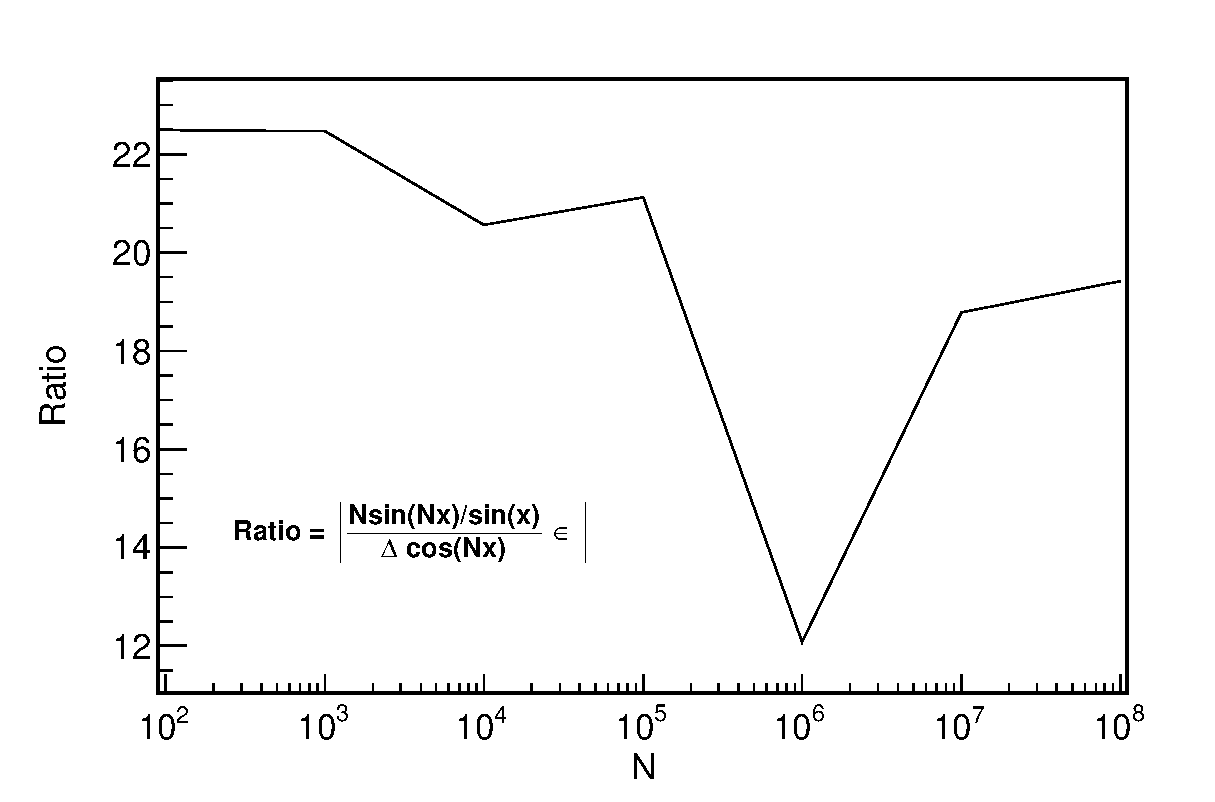
\includegraphics[width=0.5\textwidth]{figures/1a_ratio.eps}
  \hfill
  \caption{Figures for part (a) of problem 1. For each graph $x = 10^{-6}$.}
\end{figure}\\
\indent The formula given by equation (2) of the problem set does not include errors from the finite representation of intermediate steps in the recursion. The formula to include the errors would be XXXXXXXXXXXXXXX\\
\indent If use a different accuracy for the initial value of $\cos x$ and for steps in the recursion we observe an interesting effect on the propogation of error through recursion XXXXXXXXXX
\section{Problem 2}
I modified the \verb|real_time_clock.c| program to calculate the 8 operations. For each operation the program starts the clock, iterates 1000 times, stops the clock, then prints to the screen the difference in time in nanoseconds. At the end of the program, I calculate the overhead to start and stop the clock. A python script, \verb|two.py|, executes the modified clock program and captures the output. For each operation the python script computes the time it takes the complete one operation by dividing by the number of iterations. The script then runs the clock program 1000 times and histograms time required to complete one operations. The histograms indicate the variability between program executions. In the histograms below, the red shaded histogram represents {\bf no} compiler optimization and blue the {\bf highest} optimization. The number of entries in each histogram is 1000.
\begin{figure}[h]
  \centering
  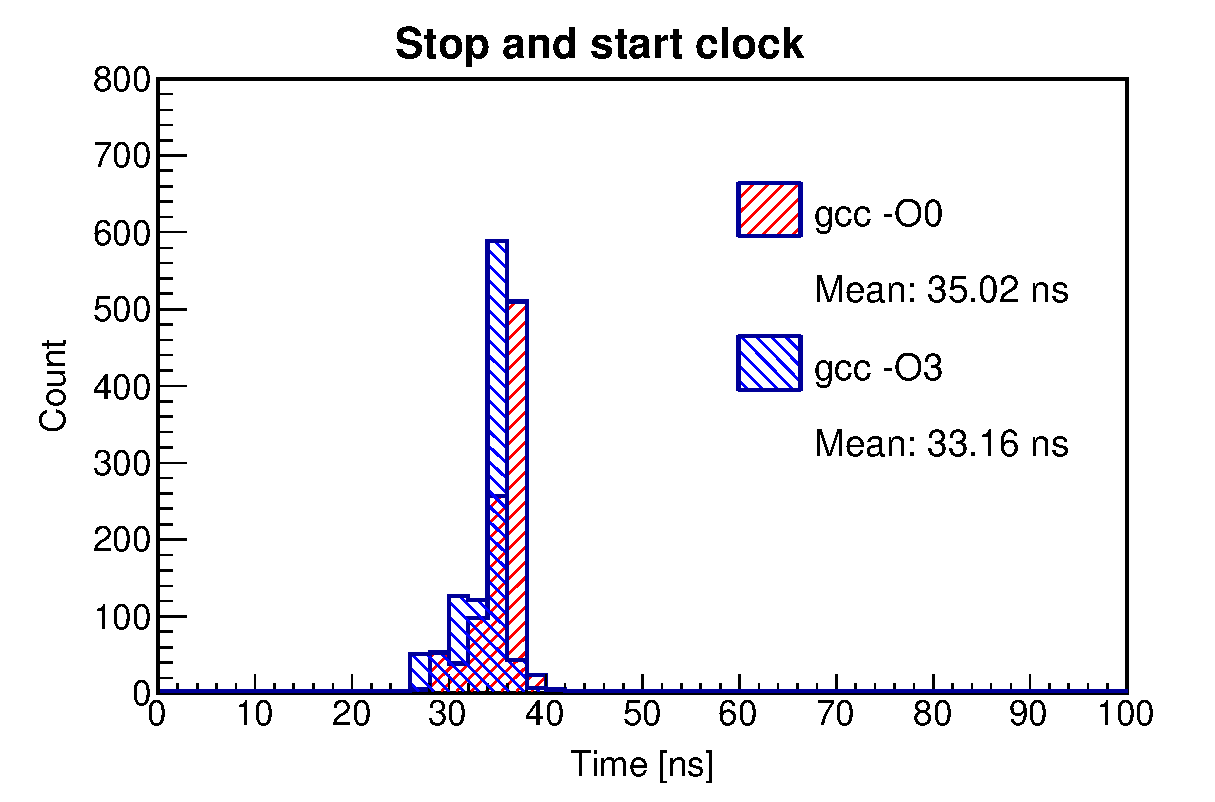
\includegraphics[width=0.5\textwidth]{figures/clock.eps}
  \subfloat[][]{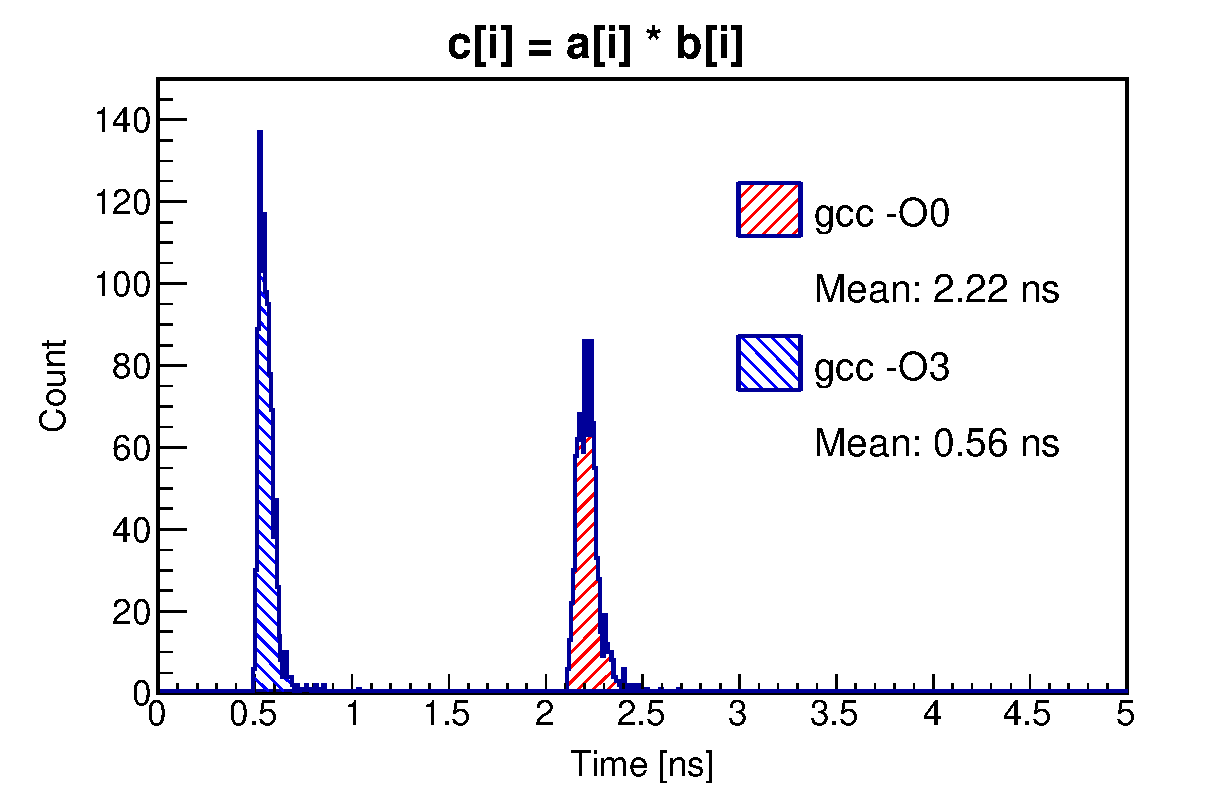
\includegraphics[width=0.5\textwidth]{figures/2_a.eps}}
  \subfloat[][]{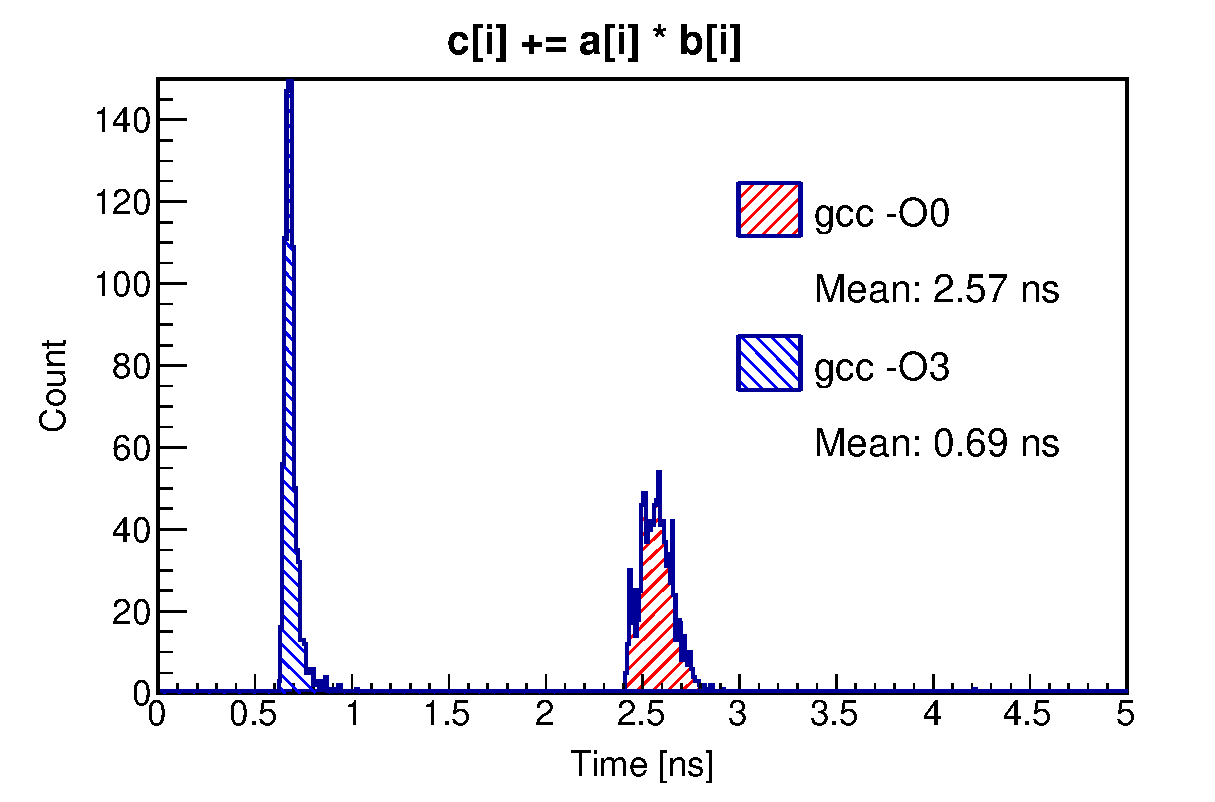
\includegraphics[width=0.5\textwidth]{figures/2_b.eps}}\\
  \subfloat[][]{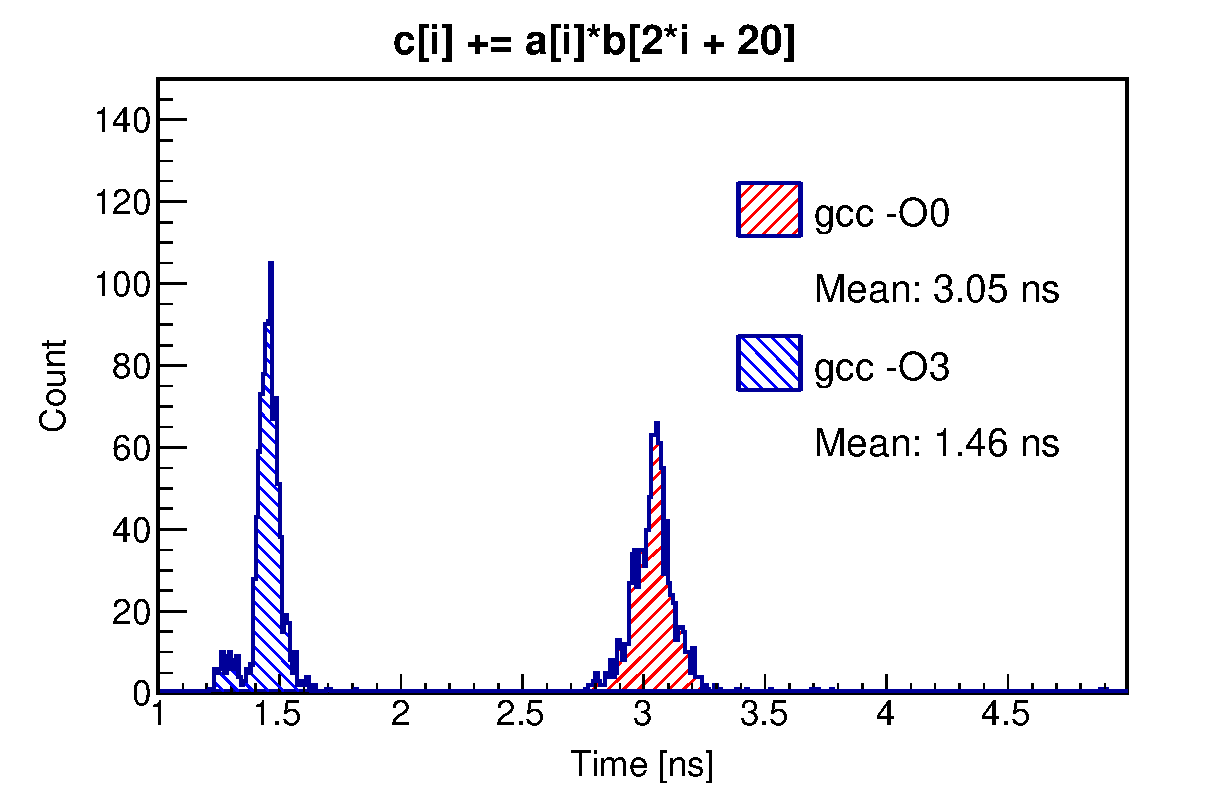
\includegraphics[width=0.5\textwidth]{figures/2_c.eps}}
  \subfloat[][]{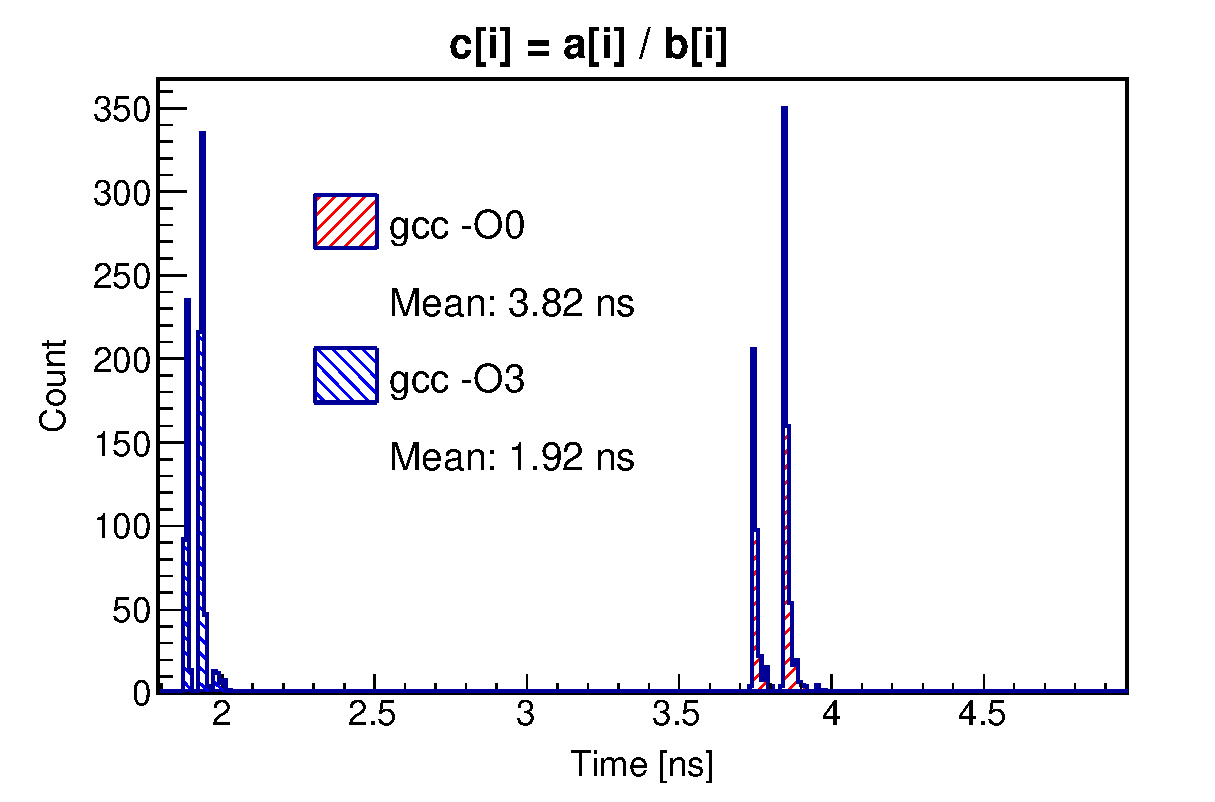
\includegraphics[width=0.5\textwidth]{figures/2_d.eps}}
\end{figure} 
\begin{figure}[h]
\ContinuedFloat
\centering
  \subfloat[][]{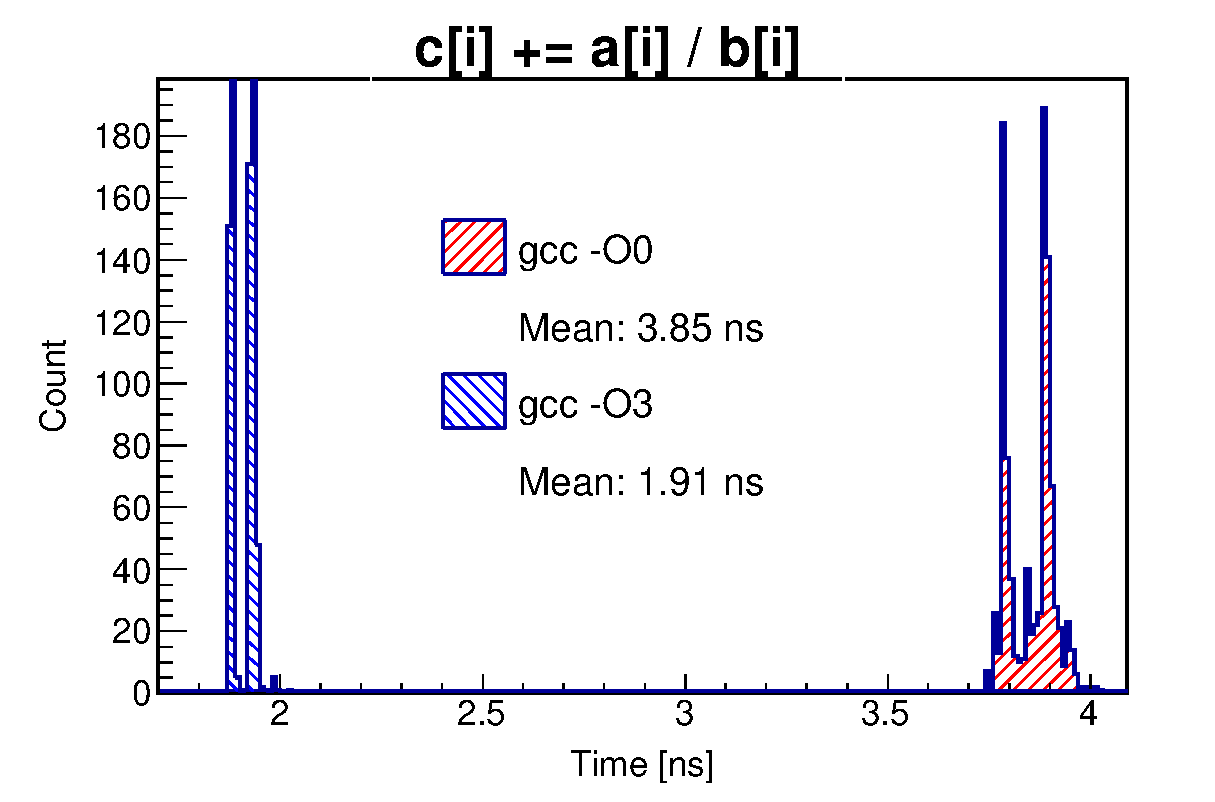
\includegraphics[width=0.5\textwidth]{figures/2_e.eps}}
  \subfloat[][]{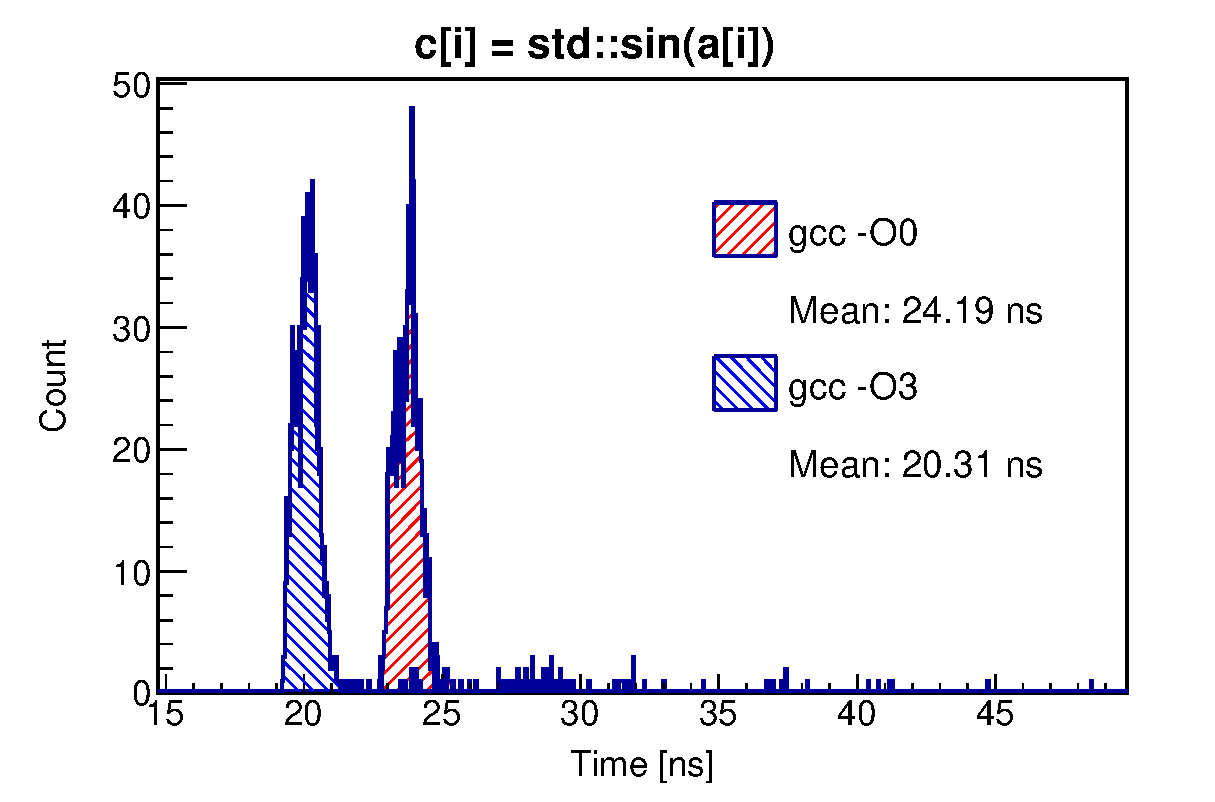
\includegraphics[width=0.5\textwidth]{figures/2_f.eps}}\\
  \subfloat[][]{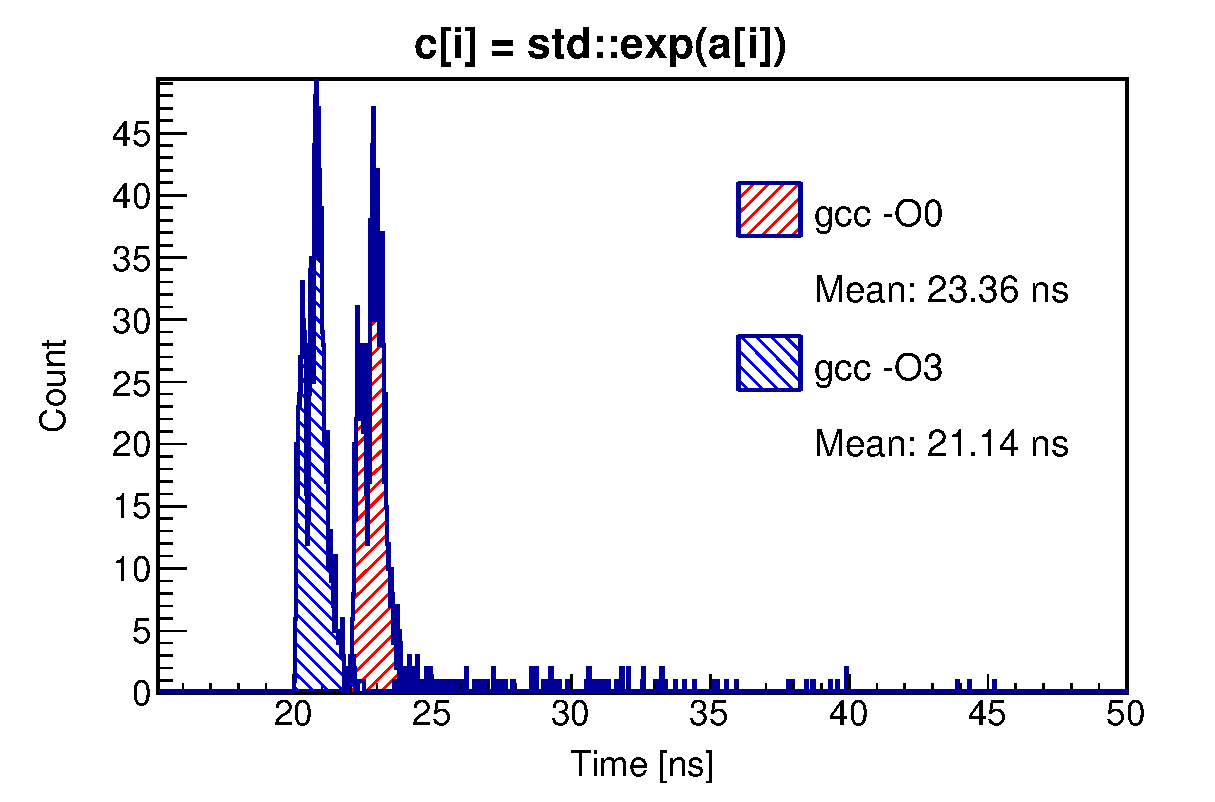
\includegraphics[width=0.5\textwidth]{figures/2_g.eps}}
  \subfloat[][]{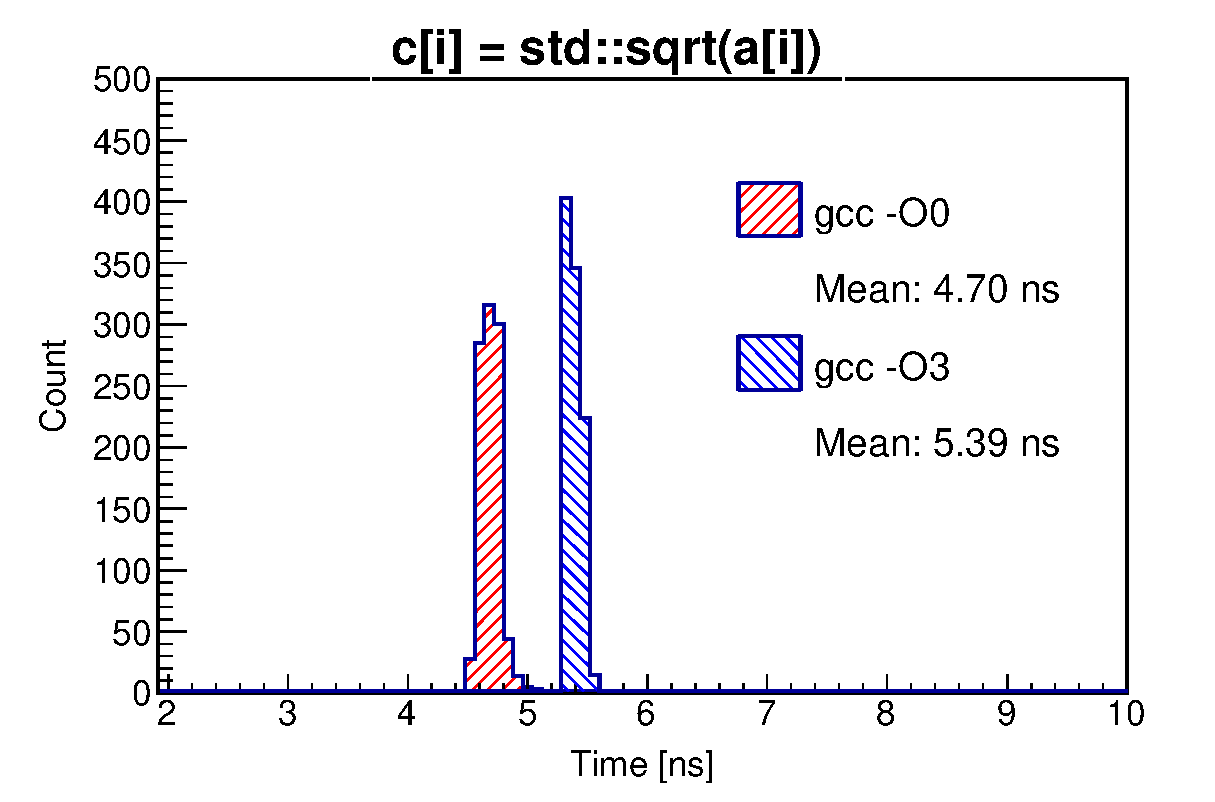
\includegraphics[width=0.5\textwidth]{figures/2_h.eps}}
\end{figure}\\
\indent The overhead required to start and stop the clock was about 35 ns as shown in the first plot and did not depend too much on the compiler optimization. The fastest operation was multiplication, depending heavily on the compiler optimization which execution speed as low as half a nano-second. The slowest operations where \verb|std::sin|, and \verb|std::exp| coming in at 20-30 ns.
\clearpage
\section{Problem 3}
The modified bessel functions of the first kind $I_2(x)$ are computed for values of $x\in\{1,2,\dots,10\}$. The program \verb|Bessel| uses the C++ boost library to call the ``true'' value of the modified bessel function \verb|boost::math::cyl_bessel_i|. The program also uses variable recursion to calculated $I_2(x)$ for different value of $x$. The \verb|Bessel| program is compiled into a shared object and loaded into python via the ROOT framework. This way, python can invoke Bessel member methods at compiled speed. The python program \verb|use.py| iterates the calculation of $I_2$ for 50 recurance steps and over 10 values of $x$. The results are plotted in the figure below. 
\begin{figure}[h]
\centering
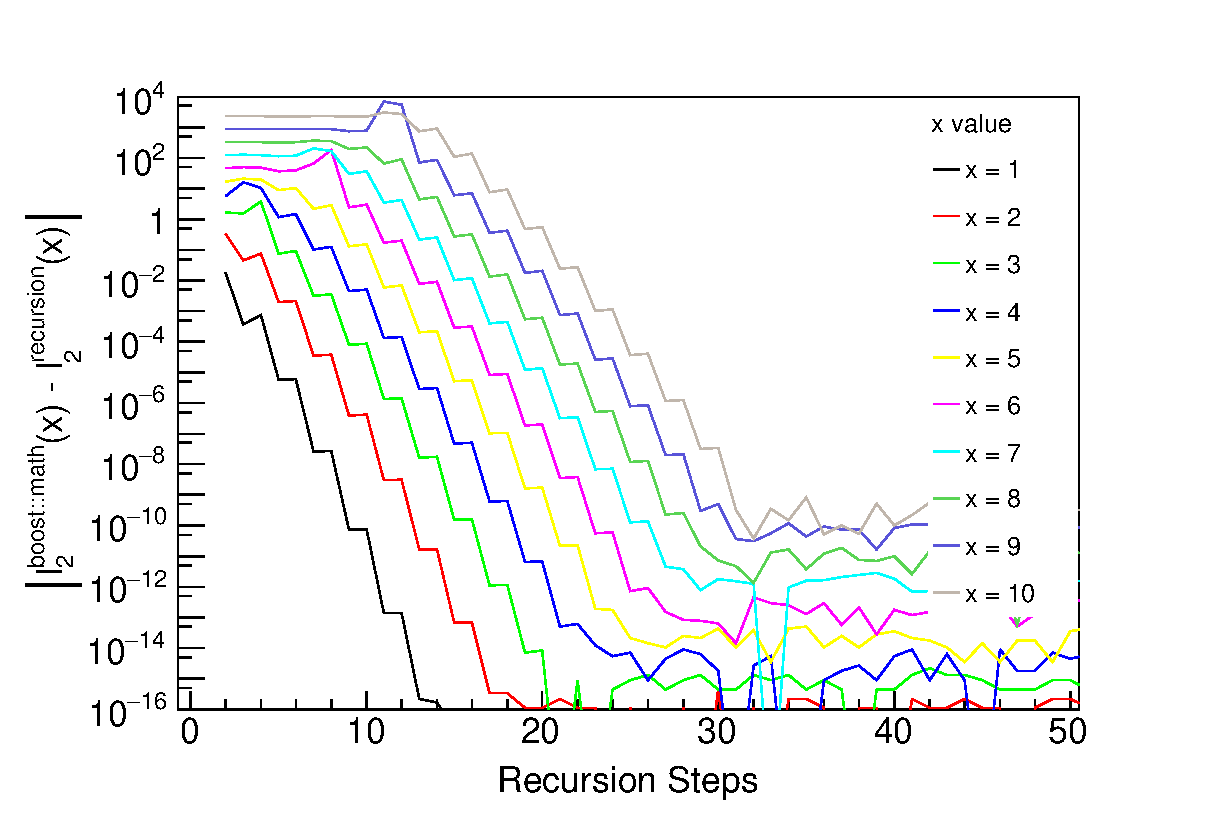
\includegraphics[width=0.6\textwidth]{figures/modified_bessel.eps}
\end{figure}\\
\indent As the number of recurance steps increases, the absolute difference between the calculated value and the true (precision of $10^{-15}$) value decreases until they agree with in IEEE double precision. Larger value of $x$ require more recurance steps to achieve higher precision. In addition, the agreement between the two values tends to level off about IEEE double precision.
\end{document}
